
\documentclass{article}
\usepackage[T1]{fontenc}
\usepackage[margin=2cm]{geometry}
\usepackage{graphicx}
\usepackage{parskip} % removes paragraph indentation

\title{Zadanie 2 - Raport}
\author{Jan Stusio}
\date{Marzec 2024}

\begin{document}

\maketitle

\section{Wstęp}

Celem zadania jest zaimplementowanie algorytmu ewolucyjnego, który jest bezgradientową metodą optymalizacji.


Analizowane tą metodą zostaną funkcje:

1. Rastrigina(https://www.sfu.ca/~ssurjano/rastr.html),

dla zakresu $x \in [-5,12;5,12]^2, x \in R^2$

$$
f(x) = 10d + \sum_{i=1}^{d} \left( x_i^2 - 10 \cos(2 \pi x_i) \right)
$$

2. Griewanka(https://www.sfu.ca/~ssurjano/griewank.html),

dla zakresu $x \in [-50, 50]^2, x \in R^2$

$$
f(x) =\sum_{i=1}^{d} \frac{x_i^2}{4000} - \prod_{i=1}^{d} \cos\left(\frac{x_i}{\sqrt{i}}\right) +1
$$

3. Drop-Wave(https://www.sfu.ca/~ssurjano/drop.html),

dla zakresu $x \in [-5.12, 5.12]^2, x \in R^2$

$$
g(x) = -\frac{1 + \cos\left(12 \sqrt{x_1^2 + x_2^2}\right)}{0.5(x_1^2 + x_2^2) + 2}
$$

\pagebreak

\section{Implementacja}

\subsection{Algorytm ewolucyjny}

W algorytmie ewolucyjnym zaimplementowałem następujące operatory i funkcje:

\quad1. Funkcję dopasowania $-$ oblicza odległość od minimum globalnego dla każdego osobnika w populacji

\quad2. Operator mutacji $-$ implementacja mutacji Gaussa

\quad3. Operator krzyżowania $-$ implementacja krzyżowania jednopunktowego, w którym przypisuję dzieciom średnie ważone wybranych wartości rodziców.

$$
p - potomek; \quad r - rodzic
$$
$$
p_1 [x] = \frac{r_1[x] + r_2[x]}{2}
$$
$$
p_1 [y] = \frac{r_1[y] + r_2[y]}{2}
$$
$$
p_2 [x] = \frac{r_1[y] + r_2[y]}{2}
$$
$$
p_2 [y] = \frac{r_1[x] + r_2[x]}{2}
$$

\quad4. Operator selekcji $-$ zaimplementowałem selekcję, w której wybieram $\mu$ osobników z populacji o najniższej wartości funkcji dopasowania.

Algorytm ewolucyjny działa zgodnie z sugerowanym pseudokodem w treści zadania.

\subsection{Funkcje}

Rozważam tylko wymiar $d = 2$, zatem analizowane funkcje można uprościć:

Rastrigin

$$
f(x) = 20 + x_1^2 - 10 \cos(2 \pi x_1) + x_2^2 - 10 \cos(2 \pi x_2)
$$

Griewank

$$
f(x) =\frac{1}{4000} (x_1^2 + x_2^2) - \cos\left(x_1\right) \cos\left(\frac{x_2}{\sqrt{2}}\right) + 1
$$

Drop-Wave jest zaimplementowana bez zmian.

\section{Badane parametry}

Badałem następujące wartości parametrów:

1. Rozmiar populacji:  20, 100, 500

2. Prawdopodobieństwo mutacji: 0.1, 0.5, 0.9

3. Prawdopodobieństwo krzyżowania: 0.1, 0.5, 0.9

4. Liczba pokoleń: 50, 100, 500



W trakcie badania parametrów zmieniała się tylko jedna wartość, pozostałe parametry były stałe. I przyjmowały następujące wartości:
\pagebreak

1. Rozmiar populacji: 100

2. Prawdopodobieństwo mutacji: 0.2

3. Prawdopodobieństwo krzyżowania: 0.2 dla testowania różnych wartości mutacji, 0.8 dla testowania wartości innych parametrów

\section{Wizualizacje parametrów}

W raporcie zamieszczam tylko przykładowe wizualizacje. Wybrane wizualizacje są zapisane w katalogu\\ \textit{results / selected results}, a wszystkie wyniki w katalogu \textit{results}.

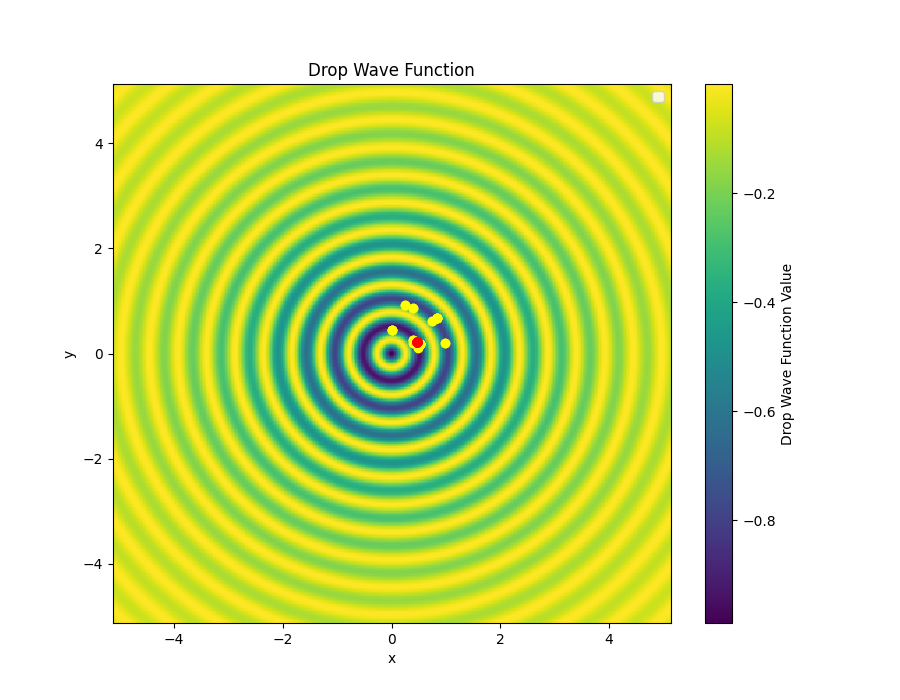
\includegraphics[width=7.7cm, height=6cm]{Drop Wave Function.png}
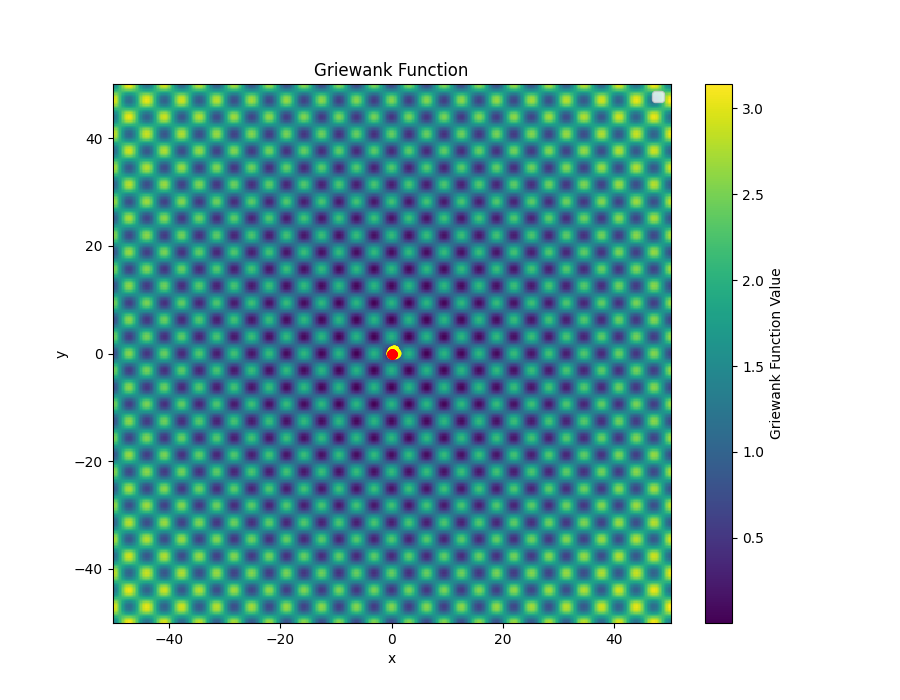
\includegraphics[width=7.7cm, height=6cm]{Griewank Function.png}

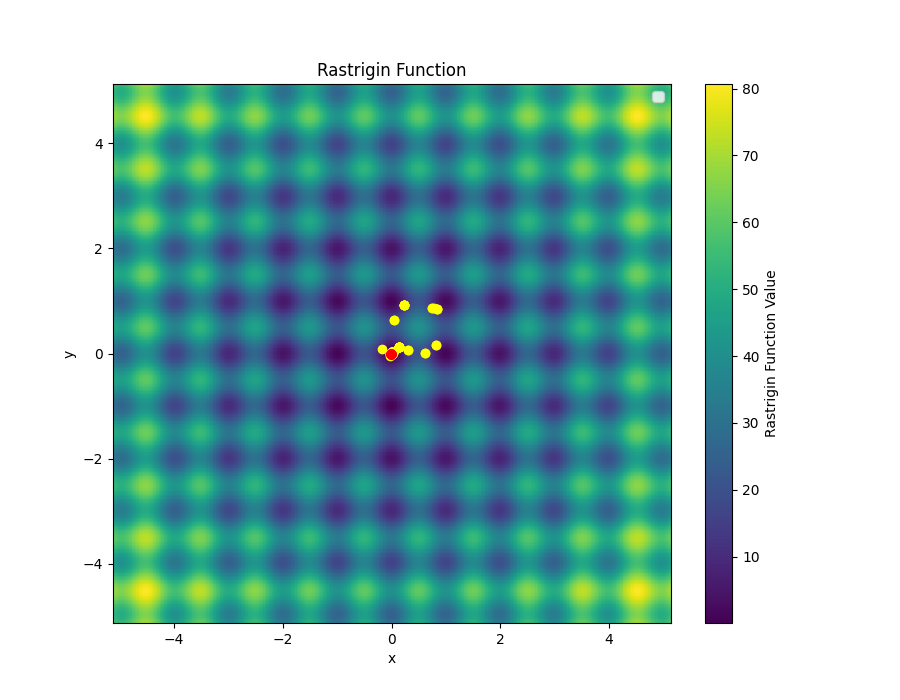
\includegraphics[width=7.7cm, height=6cm]{Rastrigin Function.png}

\section{Wnioski}

W moich testach żadna konfiguracja wartości parametrów nie była w stanie znaleźć minimum globalnego dla funkcji Drop-Wave. Najbliżej jego odkrycia była konfiguracja z prawdopodobieństwem mutacji 0.9, ale mogło się to zdarzyć przypadkowo, ponieważ populacja początkowa generowana jest pseudolosowo. Dla innych funkcji prawie każdy wynik eksperymentu kończył się odnalezieniem minimum globalnego.

Początkowa populacja generuje się w małym zakresie, blisko minumum globalnego, co przy znaczenie szerszej dziedzinie funkcji Griewank powoduje słabą eksplorację przestrzeni rozwiązań.

Moim zdaniem najciekawsze wyniki uzyskałem dla funkcji Rastrigin. Z wszystkich badanych funkcji, w tej przestrzeń rozwiązań jest najbardziej eksplorowana. W większości przypadków algorytm znalazł minimum globalne, a w przypadku, gdy nie znalazł, to znalazł minimum lokalne. W wybranych animacjach ilustrowane są przypadki, gdzie populacja znajduje się w paru 'dołkach' i ostatecznie wybiera minimum globalne. Wybrałem też przypadek dla badania parametru rozmiaru populacji, gdzie funkcja wędrowała między minimum globalnym a lokalnym i wybrała to drugie.

\end{document}
